\documentclass[tikz,border=12pt]{standalone}
\usetikzlibrary{shapes.geometric, arrows.meta, positioning, backgrounds, calc}

% ── Palette (identica all'architettura) ────────────────────────
\definecolor{canvadark}{HTML}{0D1B2A}
\definecolor{clIDE}    {HTML}{065F46}   % Firmware
\definecolor{bIDE}     {HTML}{00C9B1}
\definecolor{clAPI}    {HTML}{92400E}   % Web Research
\definecolor{bAPI}     {HTML}{F59E0B}
\definecolor{clORCH}   {HTML}{9D174D}   % Customization
\definecolor{bORCH}    {HTML}{EC4899}
\definecolor{clMEM}    {HTML}{3B4A6B}   % LLM Router
\definecolor{bMEM}     {HTML}{94A3B8}
\definecolor{clAGENT}  {HTML}{1E3A5F}   % AI Discovery
\definecolor{bAGENT}   {HTML}{3B82F6}
\definecolor{clINF}    {HTML}{7F1D1D}   % END
\definecolor{bINF}     {HTML}{EF4444}
\definecolor{clCYAN}   {HTML}{164E63}   % Integration
\definecolor{bCYAN}    {HTML}{22D3EE}
\definecolor{clPURPLE} {HTML}{4C1D95}   % STEdgeAI
\definecolor{bPURPLE}  {HTML}{A78BFA}
% ───────────────────────────────────────────────────────────────

\begin{document}
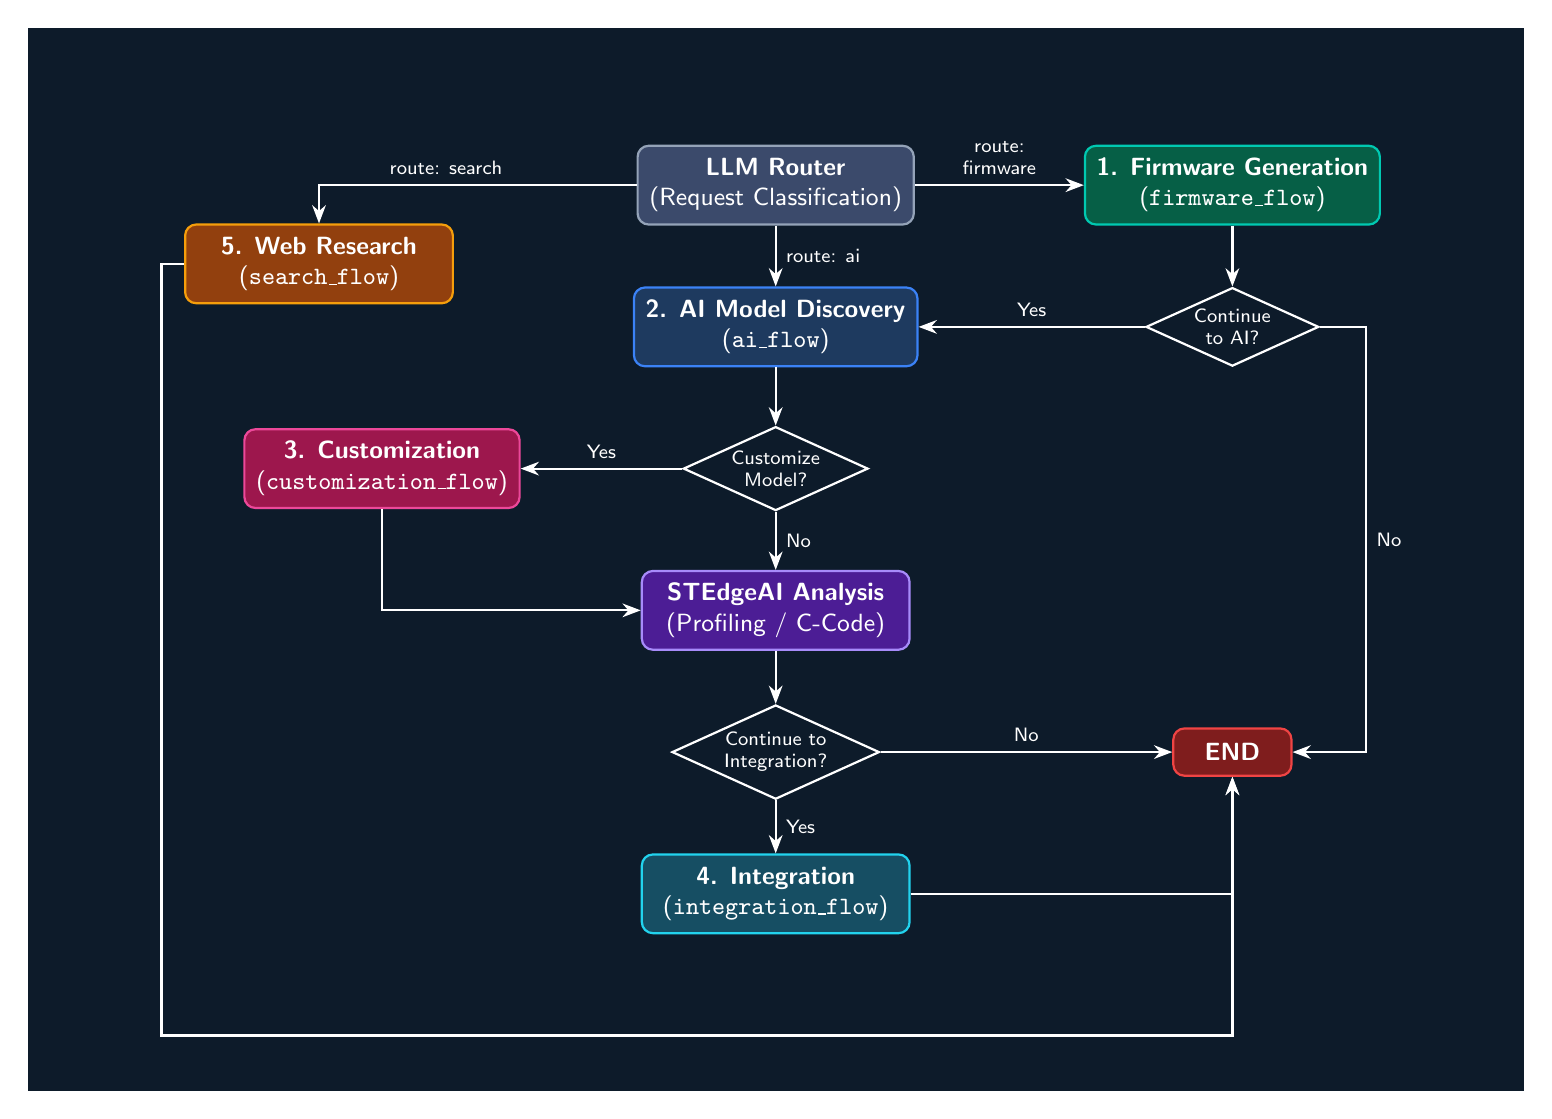
\begin{tikzpicture}[
    node distance=1.4cm and 2.2cm,
    every node/.style={font=\sffamily\small, text=white},
    wf/.style={
        draw, rounded corners,
        minimum width=3.4cm, minimum height=1cm,
        align=center, text=white,
        inner sep=0.15cm, thick
    },
    decision/.style={
        draw=white, fill=canvadark,
        diamond, minimum width=1.2cm, minimum height=0.8cm,
        align=center, inner sep=1pt, aspect=2.2,
        font=\sffamily\scriptsize, text=white, thick
    },
    arrow/.style={->, thick, >=Stealth, draw=white},
    lbl/.style={font=\sffamily\scriptsize, text=white}
]

% ── BACKGROUND ─────────────────────────────────────────────────
\begin{scope}[on background layer]
    \fill[canvadark] (-9.5, 2.0) rectangle (9.5, -11.5);
\end{scope}

% === LEFT COLUMN ===
\node[wf, fill=clAPI, draw=bAPI]
    (search) at (-5.8, -1.0)
    {\textbf{5. Web Research}\\(\texttt{search\_flow})};

\node[wf, fill=clORCH, draw=bORCH]
    (custom) at (-5.0, -3.6)
    {\textbf{3. Customization}\\(\texttt{customization\_flow})};

% === CENTER COLUMN ===
\node[wf, fill=clMEM, draw=bMEM]
    (router) at (0, 0)
    {\textbf{LLM Router}\\(Request Classification)};

\node[wf, fill=clAGENT, draw=bAGENT]
    (ai) at (0, -1.8)
    {\textbf{2. AI Model Discovery}\\(\texttt{ai\_flow})};

\node[decision, draw=white]
    (d_cust) at (0, -3.6)
    {Customize\\Model?};

\node[wf, fill=clPURPLE, draw=bPURPLE]
    (stedgeai) at (0, -5.4)
    {\textbf{STEdgeAI Analysis}\\(Profiling / C-Code)};

\node[decision, draw=white]
    (d2) at (0, -7.2)
    {Continue to\\Integration?};

\node[wf, fill=clCYAN, draw=bCYAN]
    (integration) at (0, -9.0)
    {\textbf{4. Integration}\\(\texttt{integration\_flow})};

% === RIGHT COLUMN ===
\node[wf, fill=clIDE, draw=bIDE]
    (firmware) at (5.8, 0)
    {\textbf{1. Firmware Generation}\\(\texttt{firmware\_flow})};

\node[decision, draw=white]
    (d1) at (5.8, -1.8)
    {Continue\\to AI?};

\node[wf, fill=clINF, draw=bINF,
      minimum width=1.5cm, minimum height=0.6cm]
    (endnode) at (5.8, -7.2)
    {\textbf{END}};

% ── ARROWS ─────────────────────────────────────────────────────

% Router dispatches
\draw[arrow] (router) -- 
    node[lbl, above, align=center, pos=0.5]{route:\\firmware} 
    (firmware);
\draw[arrow] (router.west) -|
    node[lbl, above, pos=0.3]{route: search}
    (search.north);
\draw[arrow] (router) -- 
    node[lbl, right]{route: ai}
    (ai);

% Firmware → Decision 1
\draw[arrow] (firmware) -- (d1);

% Decision 1 branches
\draw[arrow] (d1) -- node[lbl, above]{Yes} (ai);
\draw[arrow] (d1.east) -- (7.5, -1.8) |- 
    node[near start, lbl, right]{No}
    (endnode.east);

% AI → Customize Decision
\draw[arrow] (ai) -- (d_cust);

% Customize Decision Branches
\draw[arrow] (d_cust) -- node[lbl, above]{Yes} (custom);
\draw[arrow] (d_cust) -- node[lbl, right]{No} (stedgeai);

% Customization → STEdgeAI
\draw[arrow] (custom.south) |- (stedgeai.west);

% STEdgeAI → Decision 2
\draw[arrow] (stedgeai) -- (d2);

% Decision 2 branches
\draw[arrow] (d2) -- node[lbl, right]{Yes} (integration);
\draw[arrow] (d2) -- node[lbl, above]{No} (endnode);

% Integration → END
\draw[arrow] (integration.east) -| (endnode.south);

% Search → END
\draw[arrow] (search.west) -- (-7.8, -1.0) -- (-7.8, -10.8) -| (endnode.south);

\end{tikzpicture}
\end{document}
